\documentclass{beamer}

% ==========================================
% CONFIGURACIÓN ESTÉTICA
% ==========================================
\usetheme[progressbar=frametitle, numbering=fraction, block=fill]{metropolis}
\usecolortheme{metropolis}
\definecolor{myblue}{HTML}{005F73}
\definecolor{mygreen}{HTML}{94D2BD}
\definecolor{mygray}{HTML}{E9ECEF}
\setbeamercolor{frametitle}{bg=myblue, fg=white}
\setbeamercolor{title}{fg=myblue}
\setbeamercolor{structure}{fg=myblue}
\setbeamercolor{block title}{bg=myblue, fg=white}
\setbeamercolor{block body}{bg=mygray, fg=black}
\setbeamercolor{item}{fg=myblue}

\usepackage{graphicx}
\usepackage{booktabs}
\usepackage[T1]{fontenc}
\usepackage[utf8]{inputenc}
\usepackage[spanish]{babel}

\newcommand{\SubItem}[1]{
    {\setlength\itemindent{15pt} \item[-] #1}
}

% ============================
% DATOS
% ============================
\title{U.T. 4: Normalización de Bases de Datos}
\subtitle{Teoría, Anomalías y Formas Normales}
\author{Departamento de Informática - IES Francisco de Goya}
\date{febrero de 2026}

\begin{document}

% Portada
\begin{frame}
  \titlepage
\end{frame}

% ============================
% 1. INTRODUCCIÓN
% ============================
\section{1. Introducción y Necesidad}

\begin{frame}
  \frametitle{¿Por qué Normalizar?}
  Al diseñar una base de datos (pasando de E/R a Relacional o directamente), podemos cometer errores de diseño.
  
  \vspace{1em}
  La \textbf{Normalización} es una técnica formal para organizar los datos que nos ayuda a:
  \begin{itemize}
      \item Detectar errores en el diseño.
      \item Corregir estructuras defectuosas.
      \item Asegurar propiedades deseables en el esquema.
  \end{itemize}

  \begin{block}{Principio Básico del Diseño}
    \centering
    \textbf{"Hechos distintos se deben almacenar en objetos distintos"}
  \end{block}
\end{frame}
\begin{frame}
  \frametitle{Ejemplo: Mala Normalización}
  \textit{Problema: Una tabla con redundancias (Autor, Nacionalidad, Libro... todo junto).}
  

  %%% Datos de la tabla: SACAR DEL MD.


\begin{center}
  \resizebox{0.9\textwidth}{!}{
  \begin{tabular}{llllll}
    \toprule
    \textbf{Autor} & \textbf{Nacional.} & \textbf{ISBN} & \textbf{Título} & \textbf{Editorial} & \textbf{Año} \\
    \midrule
    Pérez Martín & Española & 7445 & Bases de Datos & Mc. Graw-Hill & 1998 \\
    Pérez Martín & Española & 8458 & Lenguaje C++ & Mc. Graw-Hill & 1996 \\
    Pérez Martín & Española & 5885 & El Modelo Relacional & Ra-Ma & 1995 \\
    García Sánchez & Española & 5885 & El Modelo Relacional & Ra-Ma & 1995 \\
    García Sánchez & Española & 2169 & Linux & Anaya & 1999 \\
    Cousteau & Francesa & 2169 & Linux & Anaya & 1999 \\
    Romboni & Italiana & 2169 & Linux & Anaya & 1999 \\
    \bottomrule
  \end{tabular}
  }
\end{center}
  
  \vspace{0.5em}
  Esto provoca anomalías de inserción, modificación y borrado. ¿Qué cosas pueden salir mal?
\end{frame}


\begin{frame}
  \frametitle{Problemas de un mal diseño 1/2}
  \begin{itemize}
    \item \textbf{Anomalías de inserción:} Dar de alta a un libro obliga a insertar tantas tuplas como autores tenga el libro. Además, pueden añadirse inconsistencias. ¿Qué pasa si al añadir una de esas tuplas pongo un año diferente para el mismo libro?
    \item \textbf{Anomalías de modificación:} Cambiar la editorial de un libro obliga a modificar todas las tuplas que corresponden a ese libro.
    \item \textbf{Anomalías de borrado:} Para dar de baja a un libro hay que borrar tantas tuplas como autores tenga el libro y, viceversa, para dar de baja a un autor hay que borrar tantas tuplas como libros haya escrito.
  \end{itemize}
\end{frame}

\begin{frame}
  \frametitle{Problemas de un mal diseño 2/2}
  
  \begin{itemize}
    \item \textbf{Pérdida de semántica:} No podemos almacenar información sobre un autor sobre el que no exista ningún libro en la biblioteca. Esto es debido a que el ISBN forma parte de la clave, y no puede contener valores nulos (integridad de la clave).
    \SubItem Análogamente, no podemos registrar libros con autores anónimos. Por la misma razón que antes, dado que el nombre del autor también forma parte de la clave primaria.
    \item \textbf{Pérdidas de información:} Al dar de baja a un libro, se pierde información sobre sus autores (si éstos sólo tuviesen ese libro en la BD).
    \SubItem Análogamente, al dar de baja a un autor se pierde información sobre los libros que haya escrito el sólo.
  \end{itemize}
\end{frame}


\begin{frame}
  \frametitle{Solución al Ejemplo 1}
  Si aplicamos un buen diseño, separamos las entidades:
  
  % [IMAGEN 1 del md: Solución E/R Autor-Libro]
  \begin{figure}
      \centering
      % Asegúrate de tener el archivo 'imagen1.png' en la carpeta
      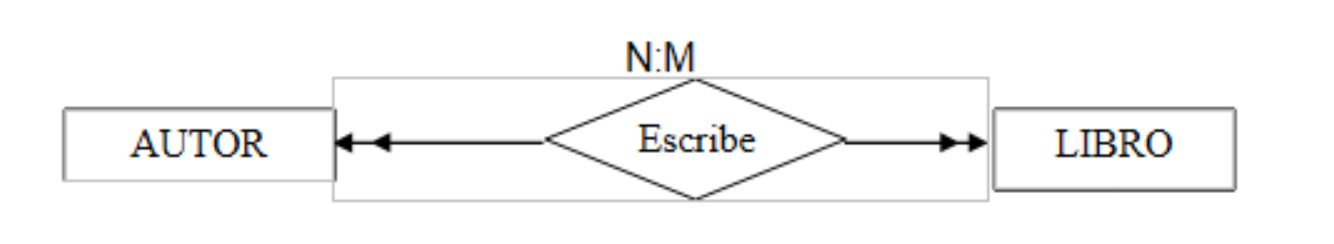
\includegraphics[width=0.7\textwidth]{imagen1.png} 
      \caption{Esquema Relacional Correcto: Autor, Libro y Escribe}
  \end{figure}
\end{frame}


\begin{frame}
  \frametitle{Solución al Ejemplo 1}
    \centering
    
    % --- Tabla de Libros ---
    \textbf{Tabla: Libro} \\
    \resizebox{0.6\textwidth}{!}{
        \begin{tabular}{llll}
            \toprule
            \textbf{ISBN} & \textbf{Título} & \textbf{Editorial} & \textbf{Año} \\
            \midrule
            7445 & Bases de Datos & Mc. Graw-Hill & 1998 \\
            8458 & Lenguaje C++ & Mc. Graw-Hill & 1996 \\
            5885 & El Modelo Relacional & Ra-Ma & 1995 \\
            2169 & Linux & Anaya & 1999 \\
            \bottomrule
        \end{tabular}
    }
    
    \vspace{0.5cm}
    
    \begin{minipage}{0.3\textwidth}
        \centering
        \textbf{Tabla: Autor} \\
        \resizebox{\textwidth}{!}{
            \begin{tabular}{ll}
                \toprule
                \textbf{Autor} & \textbf{Nacional.} \\
                \midrule
                Pérez Martín & Española \\
                García Sánchez & Española \\
                Cousteau & Francesa \\
                Romboni & Italiana \\
                \bottomrule
            \end{tabular}
        }
    \end{minipage}
    \hfill
    \begin{minipage}{0.3\textwidth}
        \centering
        \textbf{Tabla: Libro\_Autor} \\
        \resizebox{\textwidth}{!}{
            \begin{tabular}{ll}
                \toprule
                \textbf{ISBN} & \textbf{Autor} \\
                \midrule
                7445 & Pérez Martín \\
                8458 & Pérez Martín \\
                5885 & Pérez Martín \\
                5885 & García Sánchez \\
                2169 & García Sánchez \\
                2169 & Cousteau \\
                2169 & Romboni \\
                \bottomrule
            \end{tabular}
        }
    \end{minipage}
\end{frame}
\end{frame}


% ============================
% 2. PRINCIPIOS
% ============================
\section{2. Principios Generales}

\begin{frame}
  \frametitle{Tablas Relacionales}
  % [IMAGEN 2 del md: TablaRelacional2.png]
  % URL original: http://upload.wikimedia.org/wikipedia/commons/thumb/a/a1/TablaRelacional2.png/450px-TablaRelacional2.png
  \begin{figure}
      \centering
      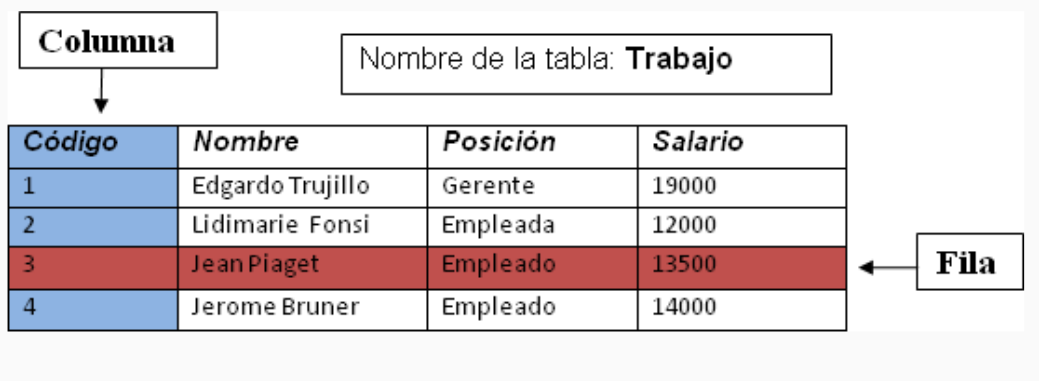
\includegraphics[width=0.5\textwidth]{imagen2.png}
      \caption{Estructura de una tabla relacional}
  \end{figure}

  La normalización distribuye campos en tablas relacionadas para:
  \begin{itemize}
      \item Evitar redundancia.
      \item Proteger la integridad de datos.
      \item Facilitar el mantenimiento.
  \end{itemize}
\end{frame}

\begin{frame}
  \frametitle{Reglas de Oro}
  Para evitar los problemas anteriores, aplicamos estas reglas:
  
  \begin{itemize}
      \item \textbf{Unicidad de información:} Cada campo debe contener un único tipo de información (no mezclar Nombre y Apellidos si se necesitan por separado).
      \item \textbf{Clave Principal (PK):} Cada tabla debe tener un identificador único.
      \item \textbf{Independencia:} Poder cambiar campos no clave sin afectar a otros.
      \item \textbf{Dependencia total:} Todos los datos de la tabla deben describir el "tema" de la tabla (la clave primaria) y nada más.
  \end{itemize}
\end{frame}


\begin{frame}
  \frametitle{Reglas Fundamentales}
  % [IMAGEN 3 del md: Ilustración decorativa sobre reglas/estructura]

          \begin{figure}
              \centering
              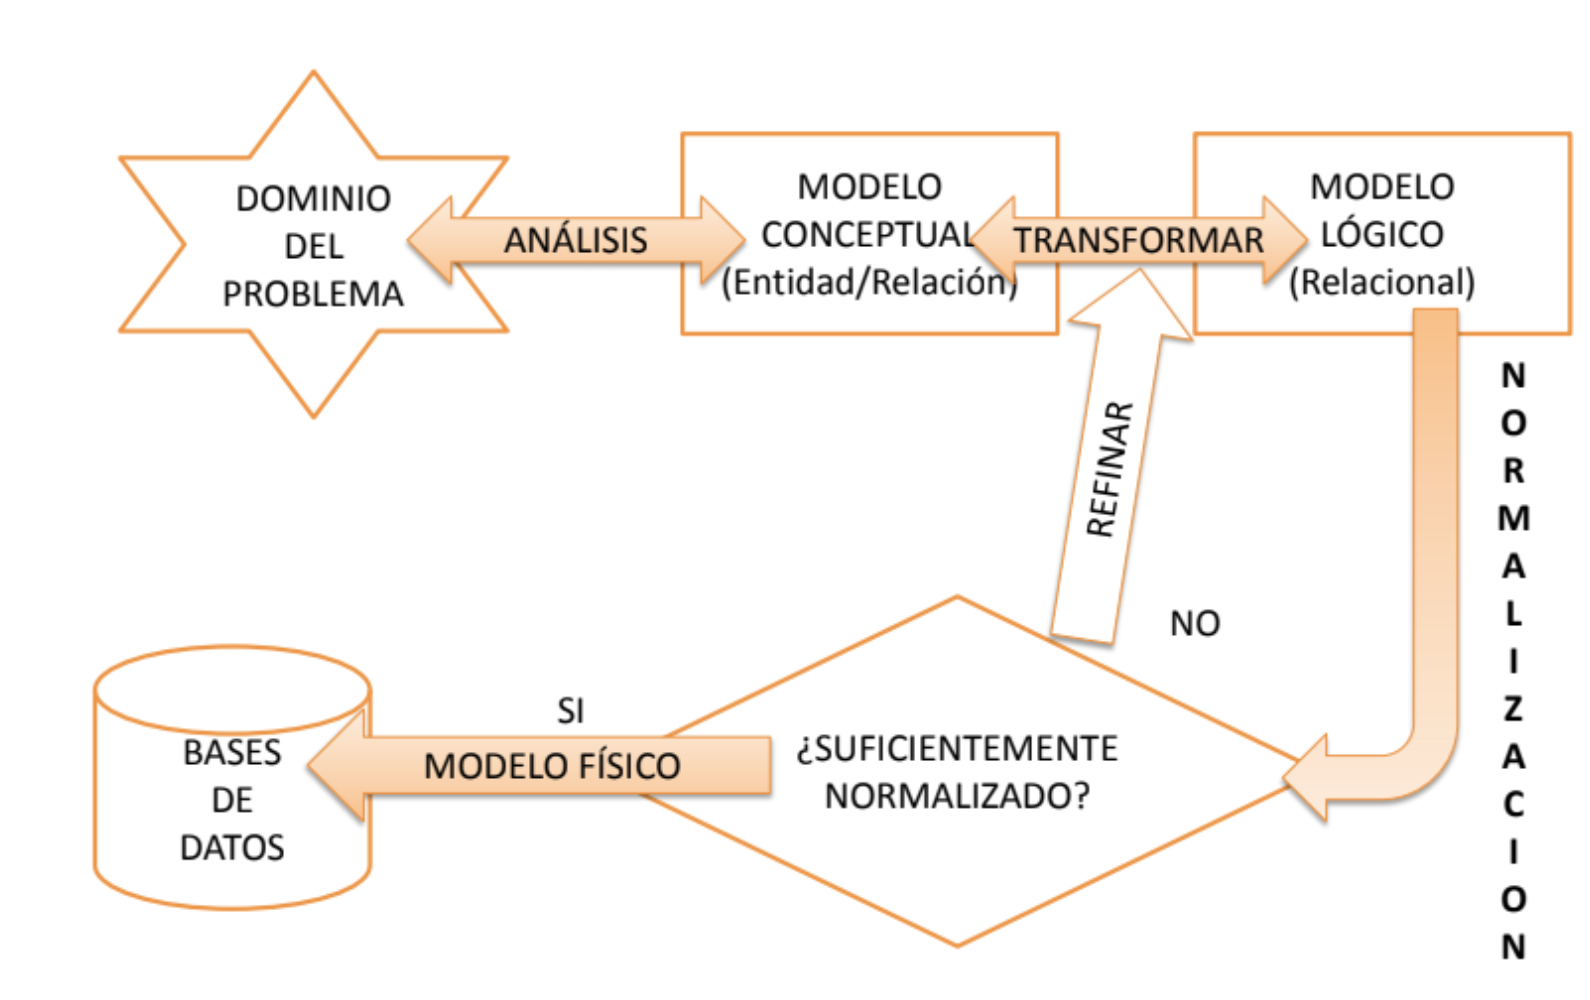
\includegraphics[width=\textwidth]{imagen3.png}
          \end{figure}

\end{frame}

% ============================
% 3. DEPENDENCIAS
% ============================
\section{3. Dependencias Funcionales}

\begin{frame}
  \frametitle{¿Qué es una Dependencia Funcional?}
  
  Dados dos atributos $A$ y $B$, decimos que $B$ depende funcionalmente de $A$ ($A \to B$) si:
  \begin{quote}
      Para cada valor de $A$ existe un valor de $B$, y solo uno, asociado con él.
  \end{quote}
  
  \vspace{1em}
  \textbf{Ejemplo:}
  $$ DNI \to Nombre $$
  (Si sé el DNI, sé el Nombre. El nombre no puede variar para un mismo DNI).
\end{frame}


\begin{frame}

  \frametitle{Ejemplo: Préstamos de Biblioteca 1/2}
    \texttt{Prestamos (\underline{Cód\_Libro}, Título, Editorial, \underline{Num\_Socio}, Nombre, Domicilio, FechaPréstamo, FechaDevolución)} 
\end{frame}

  
  \begin{frame}
  \frametitle{Ejemplo: Préstamos de Biblioteca 2/2}
  % [IMAGEN 5 del md: Diagrama de dependencias préstamos]
  \begin{figure}
      \centering
      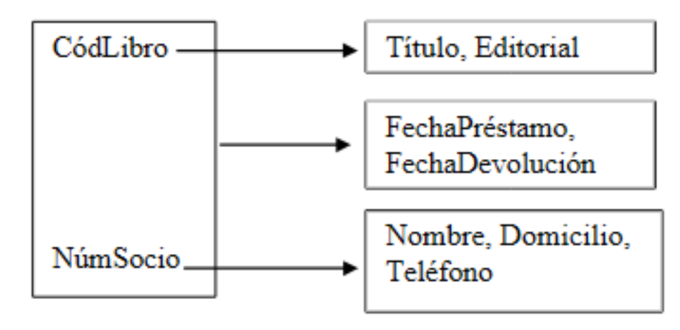
\includegraphics[width=0.7\textwidth]{imagen5.png}
      \caption{Diagrama de Dependencias Funcionales}
  \end{figure}
  
  \begin{itemize}
      \item Cód\_Libro $\to$ Título, Editorial.
      \item Num\_Socio $\to$ Nombre, Domicilio.
      \item (Cód\_Libro, Num\_Socio) $\to$ FechaPréstamo, FechaDevolución
  \end{itemize}
\end{frame}


% ============================
% Diapositiva: Dependencia Funcional Completa
% ============================
\begin{frame}
  \frametitle{Dependencia Funcional Completa}
  \begin{block}{Definición}
    Sea un atributo $X$ compuesto ($X_1, X_2$). Se dice que $Y$ tiene \textbf{dependencia funcional completa} respecto a $X$ si depende de $X$ en su totalidad, y no de $X_1$ ni de $X_2$ por separado.
    $$ X \Rightarrow Y $$
  \end{block}

  \begin{exampleblock}{Ejemplo: ¿Dependencias funcionales completas de la PK?}
    \texttt{Prestamos (\underline{Cód\_Libro}, Título, Editorial, \underline{Num\_Socio}, Nombre, Domicilio, FechaPréstamo, FechaDevolución)} 

  \end{exampleblock}
  
  \textbf{Regla de Oro:} En una tabla, todos los atributos deben tener una dependencia funcional completa de la clave principal.
\end{frame}

\begin{frame}
  \begin{exampleblock}{Ejemplo: ¿Dependencias funcionales completas de la PK?}
    \texttt{Prestamos (\underline{Cód\_Libro}, Título, Editorial, \underline{Num\_Socio}, Nombre, Domicilio, FechaPréstamo, FechaDevolución)} 

    \textbf{(\underline{Cód\_Libro}, \underline{Num\_Socio}) $\Rightarrow$ FechaPréstamo, FechaDevolución}

    \textbf{(\underline{Cód\_Libro}, \underline{Num\_Socio}) $\not\Rightarrow$ Título}

    \textbf{(\underline{Cód\_Libro}, \underline{Num\_Socio}) $\rightarrow$ Título}
  \end{exampleblock}
  
  \textbf{Regla de Oro:} En una tabla, todos los atributos deben tener una dependencia funcional completa de la clave principal.
\end{frame}

% ============================
% Diapositiva: Dependencia Funcional Transitiva
% ============================
\begin{frame}
  \frametitle{Dependencia Funcional Transitiva}

  \begin{block}{Definición}
    Sean $X, Y, Z$ atributos de una misma entidad. Se dice que $Z$ depende transitivamente de $X$ si:
    $$ X \to Y \quad \text{y} \quad Y \to Z $$
    \small{(Suponiendo que $X$ no depende de $Y$).}
  \end{block}

  \begin{exampleblock}{Ejemplo: Permiso de Conducir}
    \begin{itemize}
        \item \textbf{1.} $FechaNacimiento \to Edad$ \\
        (Sabiendo la fecha, sabemos la edad exacta).
        
        \item \textbf{2.} $Edad \to Conducir$ \\
        (La edad determina legalmente si se puede conducir).
        
        \item \textbf{Conclusión:} $FechaNacimiento \to Conducir$ \\
        (Indirectamente, la fecha de nacimiento determina si puedes conducir).
    \end{itemize}
  \end{exampleblock}

\end{frame}


\begin{frame}
  \frametitle{Tipos de Dependencia}
  \begin{block}{Dependencia Funcional Completa}
      Un campo depende de \textbf{toda} la clave primaria, no solo de una parte.
  \end{block}
  
  \begin{block}{Dependencia Transitiva}
      % [IMAGEN 6 del md: DependenciaFunional2.png (Transitiva)]
      % URL: http://upload.wikimedia.org/wikipedia/commons/thumb/3/36/DependenciaFunional2.png/375px-DependenciaFunional2.png
      \centering
      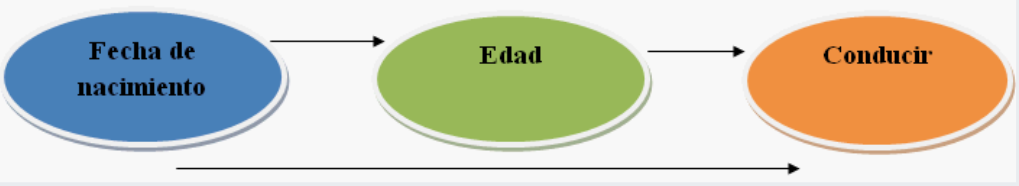
\includegraphics[width=0.5\textwidth]{imagen6.png}
      
      $ X \to Y \to Z $
      \\ Z depende de X a través de Y.
  \end{block}
\end{frame}

% ============================
% 4. FORMAS NORMALES
% ============================

\section{4. Formas Normales}
% ============================
% 1FN: Definición y Problema
% ============================
\begin{frame}
  \frametitle{Primera Forma Normal (1FN)}

  \begin{alertblock}{Definición}
    Una tabla está en 1FN si \textbf{no admite atributos multivaluados}.
    \\ Es decir, cada celda debe contener un único valor atómico.
  \end{alertblock}

  \vspace{0.5em}
  \textbf{Ejemplo de Violación (Tabla NO Normalizada):}
  \begin{center}
    \resizebox{\textwidth}{!}{
    \begin{tabular}{llllllll}
      \toprule
      \textbf{NPed} & \textbf{Fecha} & \textbf{CodC} & \textbf{Nom} & \textbf{CodArt} & \textbf{Cant.} & \textbf{Desc.} & \textbf{Pre.} \\
      \midrule
      123 & 19/11 & C14 & Pepe & A03,A15 & 24,10 & Lápiz,Goma & 25,15 \\
      145 & 24/11 & C67 & Juan & A02,A15 & 1000,10 & Folio,Goma & 1,15 \\
      \bottomrule
    \end{tabular}
    }
  \end{center}
  \footnotesize{\textit{* Nota cómo los artículos están separados por comas en una misma celda.}}
\end{frame}

% ============================
% 1FN: Procedimiento
% ============================
\begin{frame}
  \frametitle{¿Cómo pasar a 1FN?}

  Para corregir la tabla anterior, seguimos estos pasos:

  \begin{enumerate}
      \item \textbf{Identificar} los atributos que se repiten (multivaluados) para una misma clave.
      \item \textbf{Separar:} Crear una nueva tabla con esos atributos, eliminándolos de la original.
      \item \textbf{Nueva Clave:} La clave principal de la nueva tabla será la concatenación de:
      $$ \text{Clave Original} + \text{Clave del Atributo Repetido} $$
  \end{enumerate}
\end{frame}

% ============================
% 1FN: Solución
% ============================
\begin{frame}
  \frametitle{Solución: Tablas Normalizadas}

  \textbf{1. Tabla PEDIDOS} (Datos únicos por pedido)
  \begin{center}
  \resizebox{0.7\textwidth}{!}{
    \begin{tabular}{llll}
      \toprule
      \textbf{NPed (PK)} & \textbf{Fecha} & \textbf{Cod\_Cli} & \textbf{Nom\_Cli} \\
      \midrule
      123 & 19/11/96 & C14 & Pepe \\
      145 & 24/11/96 & C67 & Juan \\
      \bottomrule
    \end{tabular}
  }
  \end{center}

  \textbf{2. Tabla PED\_ART} (Desglose de artículos)
  \begin{center}
  \resizebox{0.9\textwidth}{!}{
    \begin{tabular}{llllll}
      \toprule
      \textbf{NPed (PK)} & \textbf{CodArt (PK)} & \textbf{Cant.} & \textbf{Desc.} & \textbf{Precio} \\
      \midrule
      123 & A03 & 24 & Lápiz & 25 \\
      123 & A15 & 10 & Goma & 15 \\
      145 & A02 & 1000 & Folio & 1 \\
      145 & A05 & 10 & Goma & 15 \\
      \bottomrule
    \end{tabular}
  }
  \end{center}
  \tiny{* Nota: La clave de la segunda tabla es compuesta (NPed + CodArt) para evitar duplicados.}
  \tiny{** Pregunta: ¿Qué pasa aquí con las dependencias funcionales?}
\end{frame}

% ============================
% 2FN: Definición
% ============================
\begin{frame}
  \frametitle{Segunda Forma Normal (2FN)}

  \begin{alertblock}{Definición}
    Una relación está en 2FN si:
    \begin{itemize}
        \item Está en \textbf{1FN}.
        \item Todos los atributos que no son clave dependen de \textbf{toda} la clave principal (Dependencia Funcional Completa).
    \end{itemize}
  \end{alertblock}

  \vspace{1em}
  \textbf{¿Qué significa esto?}
  \begin{itemize}
      \item No pueden existir \textbf{dependencias parciales} (atributos que dependan solo de una parte de la clave).
      \item \textit{Nota:} Si la clave principal es simple (un solo campo), la tabla ya está automáticamente en 2FN (si cumple 1FN).
  \end{itemize}
\end{frame}

% ============================
% 2FN: Ejemplo Problema
% ============================
\begin{frame}
  \frametitle{Ejemplo: Tabla NO Normalizada}

  Supongamos una tabla de notas.
  \\ \textbf{Clave Principal (PK):} \texttt{(COD\_AL, COD\_ASIG)}

  \begin{center}
    \resizebox{\textwidth}{!}{
    \begin{tabular}{lllllll}
      \toprule
      \textbf{COD\_AL} & \textbf{NOM\_AL} & \textbf{TF\_AL} & \textbf{COD\_ASIG} & \textbf{NOTA} & \textbf{CURSO} & \textbf{HORAS} \\
      \midrule
      1111 & Pepe Pérez & 911234567 & LMSI & 6 & 1ASIR & 4 \\
      1111 & Pepe Pérez & 911234567 & SSOO & 7 & 1ASIR & 8 \\
      2222 & Ana López & 912345678 & LMSI & 8 & 1ASIR & 4 \\
      2222 & Ana López & 912345678 & SSOO & 5 & 1ASIR & 8 \\
      2222 & Ana López & 912345678 & REDES & 6 & 1ASIR & 7 \\
      3333 & Juan Gil & 913456789 & FOL & 7 & 2DAI & 2 \\
      3333 & Juan Gil & 913456789 & RET & 5 & 2DAI & 2 \\
      \bottomrule
    \end{tabular}
    }
  \end{center}
  
  \vspace{0.5em}
  \small{\textbf{Problema:} Hay redundancia. Si Ana cambia de teléfono, hay que actualizar 3 filas.}
\end{frame}

% ============================
% 2FN: Análisis
% ============================
\begin{frame}
  \frametitle{Análisis de Dependencias}

  Analizamos qué campos dependen de la clave \texttt{(COD\_AL, COD\_ASIG)}:

  \begin{enumerate}
      \item \textbf{Datos del Alumno:}
      $$ \text{COD\_AL} \to \text{NOM\_AL, TF\_AL} $$
      \textcolor{red}{X Dependencia Parcial} (Solo depende de una parte de la clave).

      \item \textbf{Datos de la Asignatura:}
      $$ \text{COD\_ASIG} \to \text{CURSO, HORAS} $$
      \textcolor{red}{X Dependencia Parcial} (Solo depende de la otra parte).

      \item \textbf{La Nota:}
      $$ (\text{COD\_AL, COD\_ASIG}) \to \text{NOTA} $$
      \textcolor{mygreen}{\checkmark Dependencia Completa} (Depende de ambos: quién y en qué).
  \end{enumerate}
\end{frame}

% ============================
% 2FN: Solución
% ============================
\begin{frame}
  \frametitle{Solución: Tablas en 2FN}
  Separamos las dependencias parciales en nuevas tablas.
    \vspace{1cm}
  \begin{columns}[t]
    \begin{column}{0.3\textwidth}
      \textbf{1. ALUMNO}
      \resizebox{\textwidth}{!}{
      \begin{tabular}{lll}
        \toprule
        \textbf{COD} & \textbf{NOM} & \textbf{TF} \\
        \midrule
        1111 & Pepe & 911... \\
        2222 & Ana & 912... \\
        3333 & Juan & 913... \\
        \bottomrule
      \end{tabular}
      }
      
      \vspace{1em}
      \textbf{2. ASIGNATURA}
      \resizebox{\textwidth}{!}{
      \begin{tabular}{lll}
        \toprule
        \textbf{COD} & \textbf{CUR} & \textbf{HRS} \\
        \midrule
        LMSI & 1ASIR & 4 \\
        SSOO & 1ASIR & 8 \\
        REDES & 1ASIR & 7 \\
        FOL & 2DAI & 2 \\
        RET & 2DAI & 2 \\
        \bottomrule
      \end{tabular}
      }
    \end{column}

    \begin{column}{0.4\textwidth}
      \textbf{3. NOTAS (Relación)}
      \resizebox{\textwidth}{!}{
      \begin{tabular}{lll}
        \toprule
        \textbf{ALU} & \textbf{ASIG} & \textbf{NOTA} \\
        \midrule
        1111 & LMSI & 6 \\
        1111 & SSOO & 7 \\
        2222 & LMSI & 8 \\
        2222 & SSOO & 5 \\
        2222 & REDES & 6 \\
        3333 & FOL & 7 \\
        3333 & RET & 5 \\
        \bottomrule
      \end{tabular}
      }
    \end{column}
  \end{columns}
\end{frame}

\begin{frame}
\frametitle{Ejercicio: ¿Está en 2FN?}
  \textbf{1. Tabla PEDIDOS} (Datos únicos por pedido)
  \begin{center}
  \resizebox{0.7\textwidth}{!}{
    \begin{tabular}{llll}
      \toprule
      \textbf{NPed (PK)} & \textbf{Fecha} & \textbf{Cod\_Cli} & \textbf{Nom\_Cli} \\
      \midrule
      123 & 19/11/96 & C14 & Pepe \\
      145 & 24/11/96 & C67 & Juan \\
      \bottomrule
    \end{tabular}
  }
  \end{center}

  \textbf{2. Tabla PED\_ART} (Desglose de artículos)
  \begin{center}
  \resizebox{0.9\textwidth}{!}{
    \begin{tabular}{llllll}
      \toprule
      \textbf{NPed (PK)} & \textbf{CodArt (PK)} & \textbf{Cant.} & \textbf{Desc.} & \textbf{Precio} \\
      \midrule
      123 & A03 & 24 & Lápiz & 25 \\
      123 & A15 & 10 & Goma & 15 \\
      145 & A02 & 1000 & Folio & 1 \\
      145 & A05 & 10 & Goma & 15 \\
      \bottomrule
    \end{tabular}
  }
  \end{center}
  \tiny{Solución en pizarra.}
  
\end{frame}
% ============================
% 3FN: Definición
% ============================
\begin{frame}
  \frametitle{Tercera Forma Normal (3FN)}

  \begin{alertblock}{Definición}
    Una relación está en 3FN si:
    \begin{itemize}
        \item Ya cumple la \textbf{2FN}.
        \item \textbf{No existen dependencias transitivas.}
    \end{itemize}
  \end{alertblock}

  \vspace{1em}
  \textbf{Regla Simplificada:}
  \begin{quote}
      "Los atributos no clave deben depender únicamente de la clave, y no de otros atributos que no sean clave."
  \end{quote}
  
  \small{Si un atributo depende de otro campo que no es la clave principal, tenemos una \textbf{Dependencia Transitiva} que debemos eliminar.}
\end{frame}

% ============================
% 3FN: Ejemplo Problema
% ============================
\begin{frame}
  \frametitle{Ejemplo: Tabla con Dependencia Transitiva}

  Supongamos una tabla de Clientes.
  \\ \textbf{Clave Principal (PK):} \texttt{DNI\_CL}

  \begin{center}
    \resizebox{0.95\textwidth}{!}{
    \begin{tabular}{lllll}
      \toprule
      \textbf{DNI\_CL} & \textbf{NOM\_CL} & \textbf{DIR\_CL} & \textbf{C\_POS} & \textbf{PROV} \\
      \midrule
      1111 & Pepe Pérez & Gran Vía 17 & 28005 & Madrid \\
      2222 & Juan López & Galileo 23 & 28015 & Madrid \\
      3333 & Ana Gómez & Turia 45 & 46007 & Valencia \\
      4444 & Marta Gil & Naval 29 & 00817 & Barcelona \\
      5555 & Laura Mas & Aviación 14 & 46027 & Valencia \\
      \bottomrule
    \end{tabular}
    }
  \end{center}
  
  \vspace{0.5em}
  \small{\textbf{Problema:} Aunque la Provincia está relacionada con el Cliente (DNI_CL $\to$ Provincia), en realidad depende directamente del Código Postal (DNI_CL $\to$ C_POS $\to$ PROV.}
\end{frame}

% ============================
% 3FN: Análisis
% ============================
\begin{frame}
  \frametitle{Análisis de Dependencias (3FN)}

  Analizamos las relaciones entre los datos:

  \begin{enumerate}
      \item \textbf{Dependencia Directa (Correcta):}
      $$ \text{DNI\_CL} \to \text{C\_POS} $$
      (El DNI determina dónde vive el cliente y su código postal).

      \item \textbf{Dependencia Transitiva (Incorrecta):}
      $$ \text{C\_POS} \to \text{PROV} $$
      (La provincia depende del Código Postal, no directamente del DNI del cliente).
  \end{enumerate}

  \vspace{1em}
  \textbf{Cadena transitiva:}
  $$ \text{DNI\_CL} \to \text{C\_POS} \to \text{PROV} $$
  
  Debemos romper esta cadena separando Código Postal de Provincia.
\end{frame}

% ============================
% 3FN: Solución
% ============================
\begin{frame}
  \frametitle{Solución: Tablas en 3FN}
  Extraemos la dependencia transitiva a una nueva tabla de referencia.

  \begin{columns}[t]
    \begin{column}{0.58\textwidth}
      \textbf{1. CLIENTES}
      \resizebox{\textwidth}{!}{
      \begin{tabular}{llll}
        \toprule
        \textbf{DNI} & \textbf{NOM} & \textbf{DIR} & \textbf{CP} \\
        \midrule
        1111 & Pepe & Gran Vía & 28005 \\
        2222 & Juan & Galileo & 28015 \\
        3333 & Ana & Turia & 46007 \\
        4444 & Marta & Naval & 00817 \\
        \bottomrule
      \end{tabular}
      }
    \end{column}

    \begin{column}{0.38\textwidth}
      \textbf{2. PROVINCIAS}
      \resizebox{\textwidth}{!}{
      \begin{tabular}{ll}
        \toprule
        \textbf{CP (PK)} & \textbf{PROV} \\
        \midrule
        28005 & Madrid \\
        28015 & Madrid \\
        46007 & Valencia \\
        00817 & Barcelona \\
        46027 & Valencia \\
        \bottomrule
      \end{tabular}
      }
      \vspace{1em}
    \end{column}
  \end{columns}
  \footnotesize{\textit{* Ahora PROV depende únicamente de la clave (CP) de su propia tabla.}}
\end{frame}


\begin{frame}
  \frametitle{Resumen}
  \begin{center}
      La base de datos está bien diseñada si:
      \vspace{1em}
      
      \begin{enumerate}
          \item Cada celda tiene un solo valor \textbf{(1FN)}.
          \item Todo depende de la clave, toda la clave \textbf{(2FN)}...
          \item ...y nada más que la clave \textbf{(3FN)}.
      \end{enumerate}
  \end{center}
\end{frame}

\end{document}